\documentclass[11pt,a4paper]{article}
\usepackage{mathtext}
\usepackage{cmap}
\usepackage[T1]{fontenc}
\usepackage{ucs}
\usepackage[utf8x]{inputenc}
\usepackage[english]{babel}
\usepackage[unicode,colorlinks=true, linkcolor=black]{hyperref}
\usepackage{tikz}
\usepackage{listings}
\usetikzlibrary{arrows,decorations.pathmorphing,backgrounds,positioning,fit}
\begin{document} 
\lstset{language=[Visual]C++}

\title{ShowGraph Internals.\\ \textsf{The Implementation Document}}
\author{Boris Shurygin}

\maketitle
\begin{abstract}
This document describes internal infrastructure of ShowGraph tool. ShowGraph is a simple graph editor which is capable of performing automatic layout for directed graphs. It is also capable of reading compiler dumps of control flow graphs allowing visualization of compiler IR. Currently GCC and ICC compilers are supported. This document gives a brief overview of ShowGraph's overall design and provides detailed description of the key components.
\end{abstract}
\tableofcontents
\section{Overview}
This section gives a brief overview of ShowGraph's internal structure. All the mentioned components have more detailed description in the \emph{``Key Components''} section.

As its name suggests the ShowGraph program is a tool for graph visualization. It is capable of showing graph in an interactive window and allows user to edit it, save it and load it. Additionally ShowGraph offers parsers for intermediate representation dumps of ICC and GCC compilers to extract control flow graph from them. There are two versions of ShowGraph: interactive GUI version and command-line version for rendering graph from XML representation.

The components that interact with the user directly are GUI, command line parser and compiler IR parser which is called ``frontend'' in ShowGraph project. The GUI of course is the most exposed to the user component. All graphical parts of ShowGraph are implemented inside it. It deals with things like windows, menus, buttons, toolbars and of course graphical representation of graph (we call it \emph{graph view}). GUI features are based on Qt library and graph view employs Qt's `Graphics View' framework. Nodes and Edges are implemented as subclasses of QGraphicsItem class.

Of course QGraphicsView knows nothing about graph as a data structure and would not perform 2D graph layout for us. This functionality is implemented in \emph{layout} component which places nodes and routes edges to obtain a layout for graph.

The graph representation itself is implemented in \emph{graph} component. It deals with the graph as a set of nodes and edges. A node has the lists of the predecessor and successor edges and an edge has the predecessor and successor nodes. The graph is based on low level tools such as lists and memory pools.

The Memory pools are part of the memory management framework. The only used type of memory pool at the moment is the fixed pool. This type of pool allows for fast allocation and deallocation of memory but works with entries of the same size. To create entries of different sizes one has to create a specialized pool for each size.

There are some very low-level tools like lists, assertion macros and a singleton template that are used by the other components. The Lists are a family of classes that implement doubly-liked lists with the usual prev/next pointers. 

The implementation language of the ShowGraph is C++. External dependencies are Qt 4.5 library and Microsoft's runtime library for C++. ShowGraph is in the active development process and changes rapidly. Things described in this document may change soon, but I'll try to keep the document consistent with the current state of ShowGraph sources.

\section{Key Components}
This section describes interfaces and key implementation aspects of ShowGraph's key components. Components are described in order of increasing complexity: from basic ones to the ones built above them.
\subsection{Intrusive data structures}
Several components in ShowGraph are implemented with use of intrusive data structures. These structures share one key feature: they store all pointers needed for their operation within the client objects. This is implemented via inheritance. Typical interface for these structure would be like this:
\begin{lstlisting}
/** Implementation */
class ListItem
{
    ListItem *next_p;
public:
    void setNext( ListItem *n) { next = n};
    ListItem *next() const { return next_p};
};
/** Interface */
template< class Data, class Base> class ListIface: public Base
{
public:
    Data *next() const
    {
        return static_cast< Data*>( ListItem::next())
    }
};
\end{lstlisting}
Here the ``\lstinline{class Base}'' parameter of template must be somehow derived from ListItem. To use this list user can inherit from this interface:
\begin{lstlisting}
/** Client code */
class Data: public ListIface< Data, ListItem> 
{
    int a;
public:
    void setA( int a_){ a= a_;}
	 int getA() { return a;}
};
\end{lstlisting}
Lets discuss this example in detail. Class \lstinline{ListItem} implements simple intrusive one-way connected list. If we derive user class \lstinline{Data} from \lstinline{ListItem} directly we can make use of \lstinline{setNext(...)} method. But method \lstinline{next()} returns \lstinline{ListItem *} and user have to cast it to pointer to \lstinline{Data}. That's what interface class \lstinline{ListIface} was made for. Its intent was to avoid pushing programmer, who uses the data structures to manually cast pointers in his code. Leaving out the casts makes the interface more elegant and saves a lot of effort. 

This could be achieved without separating interface from implementation. Interface of this merged structure would look like:
\begin{lstlisting}
/** Implementation */
template < class T> class ListItem
{
    T *next_p;
public:
    void setNext( T *n) { next = n};
    T *next() const { return next_p};
};
/** Client code */
class Data: public ListItem< Data> 
{
    int a;
public:
    void setA( int a_){ a= a_;}
	 int getA() { return a;}
};
\end{lstlisting}
This achieves short term goal of making intrusive list of user objects. 

Complications arise when we derive some class from \lstinline{Data} class. In this case we would have to write casts anyway:
\begin{lstlisting}
/** Client code */
class Data: public ListItem< Data> 
{
    int a;
public:
    void setA( int a_){ a= a_;}
	 int getA() { return a;}
};
/** Derived class */
class ComplexData: public Data
{
    /** Useful extending code */
public:
    ComplexData *next() const
    {
        return static_cast< ComplexData>( Data::next());
    }
};
\end{lstlisting}
Instead of doing this, separated interface can be inherited by derived class also.
\begin{lstlisting}
/** Client code */
class Data: public ListIface< Data, ListItem> 
{
    int a;
public:
    void setA( int a_){ a= a_;}
	 int getA() { return a;}
};
/** Derived class */
class ComplexData: public ListIface< ComplexData, Data>
{
    /** Useful extending code */
public:
    /** 
     * Do not need to implement container-related routines
     */
};
\end{lstlisting}

This kind of design for intrusive data structures is used for list-related classes and for graphs.

\subsection{Tools}
Tools are placed in Utils project in ShowGraph's Visual Studio solution. They are used by other components of the system and form the basement of our application's architecture. Like every other level of ShowGraph's architecture they extensively use Qt libraries.


\subsubsection{Host Abstraction}
Host abstraction is not really a piece of code in this project. It is rather a convention, that for every primitive type we use appropriate Qt type. These types are available through \lstinline{#include <QtGlobal>} directive.

\subsubsection{Asserts}
There are two types of asserts in ShowGraph: template functions throwing exceptions and macros that just die with printing line number.

Most commonly used asserts are assert macros based on Qt's \lstinline{Q_ASSERT} and \lstinline{Q_ASSERT_X}. They are \lstinline{ASSERT( bool cond)}, \lstinline{ASSERTD( bool cond)}, and \lstinline{ASSERT_XD( cond, where, what)}. The difference between 'D' version and the macros without 'D' on the end is that \lstinline{ASSERT} stays in release mode and macros like \lstinline{ASSERTD} are removed from release code. 

Some modules define their own asserts. For example memory manager uses  \lstinline{MEM_ASSERTD( cond, what)} that reports error to happen in 'Memory Manager' and describes the error.

Function-based asserts are used for checking errors that do not cause application to die immediately and can be recovered by catching exception in proper place. They are intended for use in release code. However \lstinline{assertd( bool cond)} routine can be used for debug-only asserts.

\subsubsection{Lists}
There are three kinds of lists used in ShowGraph project:
\begin{description}
\item[ListItem] is a doubly-connected list that stores pointers to client data
\item[MListItem] is an intrusive multi-list element. List number is a template parameter. Like other intrusive data structures in ShowGraph it has corresponding interface \lstinline{MListIface}.
\item[SListItem] is a specialization of \lstinline{MListItem} for single list. Its corresponding interface template is \lstinline{SListIface}.
\end{description}

All of these lists have similar interface when working with list structure. Routines \lstinline{next()} and \lstinline{prev()} allows traversing the list in default directions. Routine \lstinline{next()} returns list element in default direction and \lstinline{prev()} returns list element in reverse direction. There are also interfaces like \lstinline{peerInDir(...)} that allows writing algorithms parameterized with traverse direction. 

One can connect and element into list by invoking \lstinline{attach(...)}. Alternatively if element is created with appropriate constructor it is also connected into list.

For \lstinline{MListItem} all these routines have additional parameter that specifies the list for this operations. An example usage of this list would be:
\begin{lstlisting}
/** See sources/Utils/list_utest.cpp for this code */
#include "utils_iface.h"

/** Define the lists we use */
enum ListTypes
{
    LIST_ONE,
    LIST_TWO,
    LISTS_NUM
};
/** Derive class of linked objects */
class A: public MListIface< A, MListItem<LISTS_NUM>, LISTS_NUM>
{

};
/** Derive class from A */
class B: public MListIface< B, A, LISTS_NUM>
{

};

/** MList testing */
static bool uTestMList()
{
    B *obj1 = new B();
    B *obj2 = new B();
    B *obj3 = new B();
    obj1->attach( LIST_ONE, obj2);
    obj1->attach( LIST_TWO, obj3);
    obj2->detachAll()
    delete obj2;
    delete obj1;
    delete obj3;
    return true;
}

\end{lstlisting}

\subsubsection{Singleton}
To provide means for creating unique objects of some class the template \lstinline{Single<class Unique>} was introduced. Its implemtation is slightly different from common implementations of Singleton programming pattern. The key difference is that creation and destruction of singleton object is not automatic with Single template. There are routines \lstinline{init()} and \lstinline{deinit()} for these purposes. 

Other aspects of implementation are conventional. A pointer to unique object can be obtained via \lstinline{instance()} routine. A pointer is a static member of Single object. 

Constructors, destructor and assignment of client object should be made private and instance of Single template should be made friend of the client class.

Here is an example of singleton usage:
\begin{lstlisting}
class A;
typedef Single< A> SingleA;

/** Sample class */
class A
{
private:
    /** private constructors, assignment and destructor */
    A(){};
    A( const A&){};
    A& operator =( const A&){};
    ~A(){};
    /** Needed for singleton creation */
    friend SingleA;
};
/** static assignment of 0 to instance pointer */
SINGLETON_INSTANCE( A);    

/**
 * Test simple singleton
 */
int main()
{
    SingleA::init();

    A* a1 = SingleA::instance();
    A* a2 = SingleA::instance();
    ASSERT( areEqP( a1, a2));
    SingleA::deinit();
    return 0;
}
\end{lstlisting}

This type of singleton is intended for objects that are inexpensive to create and do not occupy a lot of critical resources. Examples may be classes that implement logging, some statistics collection. Real example can be found in memory manager class that uses singleton-based implementation of counters for memory events like allocations and deallocations.

For single object that have expensive creation and destruction and we may not need that object in runtime, this type of singleton does not suit well. We don't have a real automatically-handled singleton implementation yet.

\subsection{Memory Managment Framework}
The key principle behind ShowGraph's memory management approach is that we mostly care for objects that can exits in large quantities. These objects are likely to benefit from allocation in pools. We can also allocate other objects in pools but this is not performance critical and if we do this - that would be for the purposes of enforcing leakage detection.

\subsubsection{Pools}
A \emph{memory pool} is a technique for managing application's memory needs by providing some additional functionality over standard library routines. One piece of memory allocated by a pool is called an \emph{entry}. All memory pools in ShowGraph project share the same interface: they allow for allocation of some memory piece and for deallocation of previously allocated one. By design pools are not suited for allocating arrays of objects since some kind of pools are not able to allocate enough ammount of continuous memory ( e.g. FixedPool have chunks with fixed number of entries). That's why \lstinline{operator new[]} is prohibited for pool-stored object (\lstinline{operator delete[]} is prohibited as well). Base class that defines pool interface is located in \lstinline{Mem} namespace and looks like:
\begin{lstlisting}
class Pool
{
    public:
        /** Allocate new memory block */
        virtual void* allocate( size_t size) = 0;
        /** Free memory block */
        virtual void deallocate( void *ptr) = 0;
        /** 
          * Functionality of 'operator delete'
          * for pooled objects
          */
        virtual void destroy( void *ptr) = 0;
};
\end{lstlisting}
Member methods are named quite straightforward: \lstinline{Pool::allocate} allocates entries, \lstinline{Pool::deallocate} performs deallocation and  \lstinline{Pool::destroy} calls object's destructor before calling  \lstinline{Pool::deallocate}. Pool-controlled objects must be derived from  \lstinline{PoolObj}.
\begin{lstlisting}
/**
 * Base class for all objects allocated in pools
 */    
class PoolObj
{
  public:
    /** Default operator 'new' is disabled */
    void *operator new ( size_t size);
    /** Default operator 'delete' is disabled */
    void operator delete( void *ptr);
    /** Default operator 'new' is disabled */
    void *operator new[] ( size_t size);
    /** Default operator 'delete' is disabled */
    void operator delete[] ( void *ptr);
       
    /** Placement new */
    inline void *operator new ( size_t size, Pool* pool);
    
    /**
     * Operator 'delete' corresponding to placement new
     * WARNING: Compiler won't call this for deletion. 
     *          It is needed for freeing memory in  
     *          case of exceptions in constructor
     */
    inline void operator delete( void *ptr, Pool* pool);
    
    /** To be called by 'destroy' routine of pool class */
    virtual ~PoolObj(){};
};
\end{lstlisting}
After derivation object of user class can be created like this:
\begin{lstlisting}
class MyClass: public PoolObj
{
   /* Some useful code */        
};

void somefunc( Pool *pool)
{
    MyClass *ptr = new ( pool) MyClass();
    pool->destroy( ptr); // Calls destructor
}
\end{lstlisting}

A \emph{Fixed pool} is a pool that creates entries of the same size which is defined by pool parameter. It uses the knowledge of the entry-size for optimization of allocation/deallocation process and for simplifying the internal bookkeeping. This simplification significantly speeds up pool's operation.

Fixed pools are created by instantiation of \lstinline{FixedPool< class Data>} template which implements interface of the \lstinline{Pool} class. The template parameter ``\lstinline{class Data}'' defines the user's object type which determines the pool's entry size.

Internal implementation of a fixed pool is based on allocating memory in so-called \emph{chunks}. A \emph{chunk} is a continuous block of memory which holds a number of entries and is allocated with one call to system. The allocated memory is managed by the pool and released to system when pool doesn't need it. This policy effectively avoids calling \lstinline{malloc/free} for every entry and prevents fragmentation. \lstinline{FixedPool} class trades off compactness for quickness and uses additional info for every entry. Every entry keeps:
\begin{itemize}
\item Its own number. To calculate pointer to chunk info from pointer to entry.
\item Number of next free entry in this chunk. For speeding up the allocation.
\item Debug info like allocation/deallocation event number or ``free'' flag for checking double deallocation.
\end{itemize}
The chunks are organized in doubly-liked list to have constant time for chunk creation/destruction. Free chunks are also linked in list to speed up the allocation. 

On allocation request pool simply gets its first free chunk and returns pointer to its first entry. On deallocation, pointer to chunk is calculated from pointer to entry using its own number and entry is simply connected to the head of free entry list in the chunk. The chunk itself is enrolled in the list of free chunks if it isn't already there. If the chunk is completely empty after this deallocation it may be deleted if there are other free chunks present. Both allocation and deallocation demand constant time unless we have to allocate a new chunk or free existing empty one.

To decrease memory usage overhead the numbers in entries are effectively one byte each. Thats two byte per entry overhead if we don't align entries on 8, 16, 32 or 64 bytes. Thus memory overhead is significant if we store small objects in such a pool but for a list unit this overhead is about 25\% and for graph's node or edge it is $\sim$6.2\%.

When project is built in debug mode the pools keep track of every entry's allocation and deallocation ID. This allows programmer to put in a breakpoint if a memory leak or double-delete occurred. The conditional breakpoint should be placed in \lstinline{MemInfo::allocReg( n)} or \lstinline{MemInfo::deallocReg( n)} where 'n' should be the ID that can be obtained from suspicious entry.

\subsubsection{Smart pointers}
Smart pointers are in the process of design now. They are not used in project at the moment. They are to be used for two purposes:
\begin{itemize}
\item Dangling pointer check
\item Reference counter implementation
\end{itemize}

There are still numerous open questions to be considered in smart pointers implementation. Should they be intrusive/external? Do they need to interact with pool's functionality? Should we allow conversion of smart pointer to plain pointer? How do we support conversions between smart pointers?

\subsection{Graph Representation}
Graph representation in ShowGraph has different aspects. Of course there are classes Graph, Edge and Node, but graph representation have some more features: it has built-in support for markers and numbering of nodes and edges. It can be also dumped to an XML file and read from it.

\subsubsection{Graph, Edges and Nodes}
Graph class represents graph as a set of nodes and edges. Graph has lists of nodes and edges which can be traversed by getting graph's first node or edge and using methods \lstinline{nextNode( node)} and \lstinline{nextEdge( edge)}. 

Graph has memory pools for nodes and edges. Operators \lstinline{new} and \lstinline{delete} are can't be applied to nodes and edges (constructors are also private).  They can be created by newNode and newEdge methods of graph. To destroy node or edge object one should use deleteNode/deleteEdge methods of graph. Using graph's methods instead of direct calls of \lstinline{new} and \lstinline{delete} is not only dictated by graph's pool system but also supports memory ownership concept: nodes' and edges' memory is owned by the graph.

As one would normally expect a node has pointers to adjacent edges. These pointers are divided in two groups: predecessors and successors. At the moment Showgraph supports directed graphs only. A node also has a unique ID that is used for storing graph in XML form and for debug purposes. This id is unique for all nodes of a graph, not only the once that are living at particular point in execution but for deleted nodes also, i.e. ID is never reused. A node has pointer to the graph so it can't belong to more than one graph. Since node is a list item in graph's node list one can traverse the list with nextNode method. Adjacent edges' lists can be obtained by firstPred() and firstSucc() methods.

An edge has a predecessor and successor (let's call them ``pred'' and ``succ'' for short). Note that if some edge $e$ has successor node $n$ this edge would be predecessor of $n$ and vice versa. Like a node an edge has its unique id and pointer to graph (which is redundant since pred and succ of node are valid pointers to nodes by design and graph can be obtained from any of them).

\subsubsection{Markers and Numerations}
Every node and edge can be marked and numbered. To do this one can acquire a marker or numeration from graph. When a marker is created there are no nodes/edges in graph marked with it. This is also true for a fresh numeration. If you create new numeration there are no nodes numbered with it. Number of simultaneously alive markers/numerations is limited so they should be freed after use.

Interfaces for markers and numerations are quite similar so let's see one of them: interface for using numeration. Numeration can be obtained from `NumManager' ( graph is a subclass of it) by method \lstinline{newNum}. One use it with the subclasses of `Numbered' class to number the objects (nodes/edges or some others). Routines for this are \lstinline{isNumbered}, \lstinline{number}, \lstinline{setNumber}, \lstinline{unNumber} and \lstinline{clear}. The latter both set the number to \emph{`unknown'} value but \lstinline{unNumber} says if an object was numbered in given numeration.

On low level numerations and markers are implemented as a pair: index and value. This is done to minimize cleaning frequency. Let's see how it works.

Markers can be implemented as a simple index to an array of booleans which store information about object being marked or not. In this case we would have to clean all objects once we are done with marker or leave it to the client classes. The first would be quite expensive: it could add another $N$ multiplier to complexity of algorithms that use markers. The second one is what we tried to avoid: forcing client classes to implement a bunch of copy paste code that would manage the markers and objects marked with them.

Instead of doing this we use an \emph{index} and a \emph{value}. To check if an object is marked we see if in markers array a proper position has corresponding value. A new value is created each time we create a marker and index is selected among free positions (that's why we have limited number of markers at any given execution point). We create new value by incrementing the last created value. We wipe out dead makers after we have reached the maximum of value variable capacity and start giving values from the beginning. Numerations are implemented in the same manner.

\subsubsection{XML representation}
Graph can be stored in an XML file. The format is quite straightforward and I believe that the following example would be sufficient. This is what graph's XML representation looks like:
\begin{lstlisting}
<graph>
    <node x="-4" y="-203" id="0" label="Node 0" />
    <node x="-64" y="-103" id="1" label="Node 1" />
    <node x="50" y="-103" id="2" label="Node 2" />
    <edge target="1" source="0" />
    <edge target="2" source="0" />
</graph>
\end{lstlisting}
There are obviously two main tags: node and edge. Edge properties `target' and `source' mean `id' of successor and predecessor nodes. Node label is not a basic property of graph it is additional data of GNode (which is a node of visualized graph). Node's `x' and `y' are also properties of GNode.

Each level in graph inheritance hierarchy has its own additional properties for node and edge. Some of them can be stored in XML. At each level graph can be stored and read from XML. It won't cause an error if XML is stored by one graph. For example a visualized graph saved to XML can be read by basic graph which will ignore fields it does not recognize.

\subsubsection{Subclassing Graph}
A set of classes that behave like a ShowGraph's graph should consist of at least three classes: a representation for graph as a whole, a class for node-like objects and a class for edge-like objects. Lets call them `MyGraph', `MyNode' and `MyEdge'. These class should be derived from Graph, Node and Edge classes accordingly. Unfortunately there are more things to do before this subclasses operate as a graph. Here is the list:
\begin{itemize}
\item Predeclare MyGraph, MyNode and MyEdge
\item Make them inherent classes of Graph, Node and Edge using \emph{public} keyword
\item Declare MyGraph as a frined of MyNode and MyEdge. Declare MyNode friend of MyEdge
\item Write code for creating pools of proper size. A good place to put this is MyGraph's contructor. Graph's constructor has a boolean parameter that tells it whether it should create pools. When calling it from subclass you should call Graph's constructor with \emph{`false'}. It would be reasonable make the constructor with the boolean parameter to allow next level subclasses to prevent pools creation.
\item Implement functions createNode and createEdge so that they call operator new for MyNode and MyEdge.
\item Implement writing (and reading) of MyNode's and MyEdge's additional data to XML file.
\item Implement functions that should operate in terms of MyGraph, MyNode and MyEdge by writing static casts of result of corresponding base class functions.
\end{itemize}

The last step looks awfully awkward. A more elegant solution is found already, I'm considering using templates for this. All these steps are done in `Graph/agraph.h' which provides a fairly small and understandable  example.

\subsection{Automatic Graph Layout}
ShowGraph performs automated layout of directed graph on a plane. Layout is done via Sugiyama-like algorithm. Nodes are placed from top to bottom. Algorithm assumes that graph has a `common direction' and tries to place nodes in such a way that for most of the edges the successor is lower than the predecessor. It is implemented as a multi-step routine. The steps are:
\begin{enumerate}
\item Make list of graph's enter nodes
\item Make graph acyclic by inverting some edges. This is done by inverting graph's backedges.
\item Rank nodes, to find level of every node and insert pseudo nodes on edges that span across multiple levels. This gives us vertical position of every node.
\item Compute horizontal coordinate, wich uses barycenter heuristic to position a node close to the nodes connected with it on other levels
\end{enumerate}
Each of these steps make heuristic decisions that need tuning and require improvement. The implemented version of far from a mature layout algorithm like Graphviz's \emph{dot} (http://www.graphviz.org) or aiSee (http://aisee.de). In fact the implemented version of ShowGraph's layout method is strongly influenced by paper \emph{`A method for drawing directed graphs'} describing dot's algorithm.

\subsubsection{Finding Enters}
One of algorithm's heuristic says that nodes that do not have predecessors should be placed on topmost level in layout. This rule generally supports idea of drawing edges in downward direction. Levels of the other nodes are computed relatively to these \emph{`enter nodes'}. All nodes that are reachable from these enters can be assigned to a level basing on the distance from enter. We keep track of reachable nodes by marking them. When we find an enter node we mark all nodes that we can reach from it. In the end we should mark all the nodes in graph. The problem is that sometimes there are no nodes without predecessors or some subgraph is unreachable from the enter nodes (e.g. a loop that does not have edges going to it). In this case we can't compute levels for some nodes and have to make a heuristic decision selecting nodes that would be placed at the top.

One of the simple solutions would be to break unreachable loops by selecting random unreachable node and enrolling it into enter list. This solution can result in the placement of two connected nodes on the same level. Though we could cope with that later, it would complicate edge routing which can be a very simple procedure if we do not have to draw edges around nodes on the same level. Another effect of this is that selecting random nodes for the top we do not really support the top-down fashion of graph placement. This means that we would have to draw a lot of edges in upward direction.

If we look deeper into the problem of unreachable loops, we can see that there is a useful property of these loops. They do not have entering edges but they can have exiting edges. So there are loops that have outgoing edges and there are loops without them. 

An exit edge of the loop gives us an opportunity for better placement of nodes that became unreachable due to being successors of an unreachable loop. To do this we go upwards from nodes without successors and look for a backedges (in terms of upward traversal) of such loops and simply add its successors to enter list. This 'pseudo enter' node makes a good enter point since a loop body and loop's successors are reachable from it. These nodes then can be placed in natural top-down direction and the edge that was backedge in upward traversal will be drawn from bottom to top.

Now that we done upward traversal we have to deal with loops that do not have any enters/exits. Here our algorithm gives up and simply adds random node of such loop to enter list. Breaking infinite loop this way does not guarantee that all previously unreachable nodes will become reachable. So we add nodes reachable from our new enter and select next random node from nodes that are still unreachable. We repeat this until all nodes in graph are marked.

This method gives us such a list of enter nodes that every node is reachable from at list one enter node.

\subsubsection{Making Graph Acyclic}
Given the list of enter nodes we perform DFS to classify edges. Then we invert backedges and voil\'a, graph becomes acyclic.

\subsubsection{Ranking}
A rank of a node is its max distance from the enter nodes. It is an integral non-negative value. We start from enter nodes and assign ranks in downward pass. Every node is visited when its predecessors have been visited. The algorithm also takes in account inverted edges.

Nodes of the same rank form level. Each level has a height property which is the maximum height among its nodes. Levels are positioned vertically in order from 0 to the maximum node rank. Zero level is the topmost. Level's vertical position determines its nodes' vertical position. All nodes of a level are vertically adjusted to make their centers aligned.

For further steps edges should connect nodes that are from neighbor levels. To enforce this we insert pseudo nodes on each edge that spans across multiple levels. These pseudo nodes are used as the bending points for the long edges.

\subsubsection{Horizontal Placement}
Horizontal placement has several passes. They can be upward and downward. Depending on pass direction algorithm processes levels one by one in order of decreasing or increasing rank. First the nodes within a level form a list that is sorted according to an ordering heuristic. By now this list is sorted according to barycenter heuristic. Then nodes in the list are given coordinates. They are simply assigned coordinate that will put center of the node according right in barycenter position. The problem is that nodes can be placed too close to each other and start intersecting. Let's see an example:\\
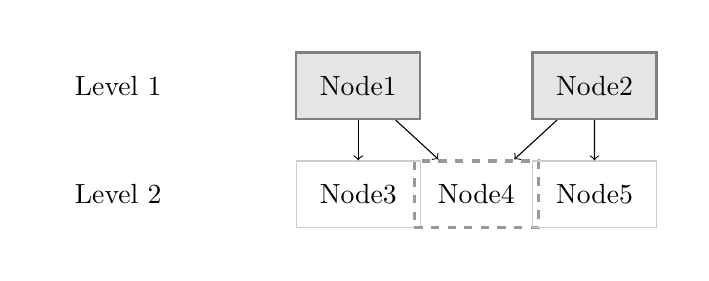
\begin{tikzpicture}
%Example of grouping	part1 
	[
	 	 %Styles
       inner sep=3mm,       
       placed_node/.style={rectangle,draw=black!50,fill=black!10,thick},
		 pending_node/.style={rectangle,draw=black!20},
		 pending_node_a/.style={rectangle,draw=black!40,dashed,very thick},
	    group_node/.style={inner sep=0.5mm, rectangle,draw=black!40,dashed},
		 label_simple/.style={rectangle}
    ]

    %Node placement
    \matrix[row sep=5mm,column sep=2mm] {
	    %Level 1
	    \node (level1)[label_simple] {Level 1}; &
       \path (0,0) ++(2,0) node (node1) [placed_node] {Node1}
	    ++(3,0) node (node2) [placed_node] {Node2}; \\
       %Level 2
	    \node (level2)[label_simple] {Level 2}; &
       \path (0,0) ++(2,0) node (node3) [pending_node] {Node3}
       ++(1.5,0) node (node4) [pending_node_a] {Node4}
       ++(1.5,0) node (node5) [pending_node] {Node5};\\
   };

   %Edges
   \path
       (node1) edge [->] (node3)
       (node1) edge [->] (node4)
       (node2) edge [->] (node5)
		 (node2) edge [->] (node4);
\end{tikzpicture}

As you can see node 4 intersects with nodes 3 and 5. To prevent this the horizontal placement algorithm uses grouping. It finds intersecting nodes and groups them. The group is placed as a whole. Its width is the sum of included nodes' widths with separations between nodes. Grouping is started with each node in its own group. Then intersecting groups are merged into new one. This new group is also tested for the intersection and merged with the others if necessary. And so on until there are no intersecting groups.\\
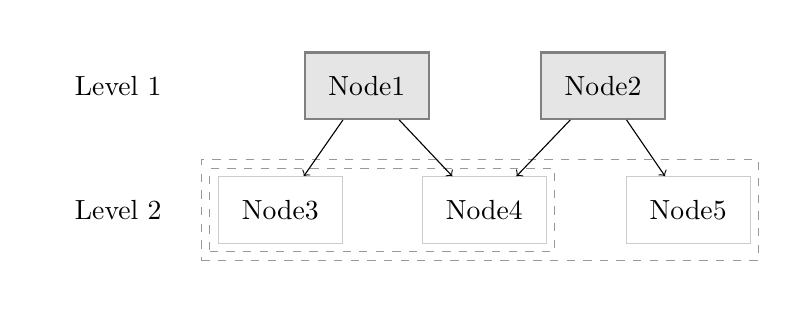
\begin{tikzpicture}
%Example of grouping	part2 
	[
	 	 %Styles
       inner sep=3mm,       
       placed_node/.style={rectangle,draw=black!50,fill=black!10,thick},
		 pending_node/.style={rectangle,draw=black!20},
		 group_node/.style={inner sep=1mm, rectangle,draw=black!40,dashed},
		 label_simple/.style={rectangle}
    ]

    %Node placement
    \matrix[row sep=5mm,column sep=2mm] {
	    %Level 1
	    \node (level1)[label_simple] {Level 1}; &
       \path ++(1.1,0) node (node1) [placed_node] {Node1}
	    ++(3,0) node (node2) [placed_node] {Node2}; \\
       %Level 2
	    \node (level2)[label_simple] {Level 2}; &
       \path node (node3) [pending_node] {Node3}
       node (node4) [pending_node, right=of node3] {Node4}
       node (node5) [pending_node, right=of node4] {Node5};
       \node (group1) [group_node, fit=(node3) (node4)] {};
		 \node (group2) [group_node, fit=(group1) (node5)] {};\\
   };

   %Edges
   \path
       (node1) edge [->] (node3)
       (node1) edge [->] (node4)
       (node2) edge [->] (node5)
		 (node2) edge [->] (node4);
\end{tikzpicture}\\
In this example first nodes 3 and 4 are grouped together. Then their group is merged with group consisting only of node5. Now nodes are placed without intersection.\\
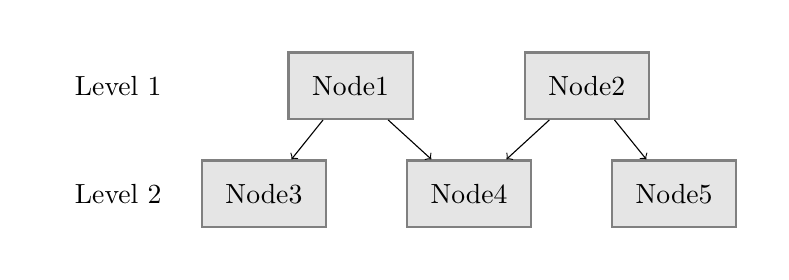
\begin{tikzpicture}
%Example of grouping	part3 
	[
	 	 %Styles
       inner sep=3mm,       
       placed_node/.style={rectangle,draw=black!50,fill=black!10,thick},
		 pending_node/.style={rectangle,draw=black!20,dashed},
		 pending_node_a/.style={rectangle,draw=black!40,dashed,very thick},
	    group_node/.style={inner sep=0.5mm, rectangle,draw=black!40,dashed},
		 label_simple/.style={rectangle}
    ]

    %Node placement
    \matrix[row sep=5mm,column sep=2mm] {
	    %Level 1
	    \node (level1)[label_simple] {Level 1}; &
       \path ++(1.1,0) node (node1) [placed_node] {Node1}
	    ++(3,0) node (node2) [placed_node] {Node2}; \\
       %Level 2
	    \node (level2)[label_simple] {Level 2}; &
       \path node (node3) [placed_node] {Node3}
       node (node4) [placed_node, right=of node3] {Node4}
       node (node5) [placed_node, right=of node4] {Node5};\\
   };

   %Edges
   \path
       (node1) edge [->] (node3)
       (node1) edge [->] (node4)
       (node2) edge [->] (node5)
		 (node2) edge [->] (node4);
\end{tikzpicture}

There are three passes of horizontal placement first downward, upward and second downward. They are done to make placement of successorless and predecessorless nodes more reasonable. At the time we run first downward pass we have to compute predecessor-less nodes' coordinates regardless of the successors' coordinates. Then when we go upwards we consider coordinates of successorless nodes instead of 0 which is result of barycenter heuristic for them. Similarly on the final pass we place predecessorless nodes accordingly to the results of the upwards pass.

\subsection{GUI Implementation}
GUI is based on the Qt libraries. Graph visualization is done by the Graphics View framework classes. Nodes and edges have QGraphicsItem subclasses to show them in QGraphicsView window. The graph view as a widget is a subclass of QGraphicsView. Other things like buttons, menus and toolbars have nothing special.

\subsection{Frontend}
Frontend supports dumps of GCC's (4th version) and ICC's intermediate representations.

It is implemented as a simple line by line parser. There are two modes of operation. First one is fast and only looks for routine names and compiler phase names. Second one looks for nodes' and edges' descriptions and builds graph from them. The node text is attached to the node as a QDocument object.

\section{Project Organization}
Currently ShowGraph is being developed for Windows using Visual Studio 2005. Therefore project is organized around VS solution. Other operating systems or build systems are not supported. This is likely to change in nearest future. There are plans of supporting Linux and using \emph{make} tool for building.

Lets see what's inside the MS VS solution. There are mainly four target projects in solution: `autodoc', `Gui', `Console' and `UnitTest'. `Autodoc' project uses \emph{Doxygen} tool to create documentation from source code. `Gui' and `Console' projects generate binaries for GUI and console versions of ShowGraph. GUI version is primary version for most users and console version is provided to enable using showgraph from console and in scripts for graph image generation. Console version is also supposed to be used in automated testing of ShowGraph's layout engine. `UnitTest' is supposed to be built and run as a sort of sanity check for tools and most packages if it exits with 0 the check is to be considered passed.


\subsection{Building}
Any of four targets can be built separately. Or one can build the whole solution to get them all.

To work with project one needs:
\begin{itemize}
\item MS Visual Studio 2005 ( or higher, but that was not tested)\
\item Subversion client. My personal favorite for Windows is TortoiseSVN http://tortoisesvn.net/
\end{itemize}

MSVS is of course `a must' at the moment as it is main development tool. There will be a choice once the projects supports gcc, make and others. SVN is needed to get the sources. Follow these steps to build the ShowGraph tools:
\begin{enumerate}
\item Install and build Qt (see http://qt.nokia.com/)
\item Checkout sources from http://showgraph.googlecode.com/svn/trunk/
\item Add Qt directories `bin', `lib', and some `include' directories to VC++ directories in MS VS options
\item Run `Build Solution' in Visual Studio
\end{enumerate}

\subsection{Testing}
Due to lack of resources the testing process in not clearly defined. Up to this moment all testing was done by hand of developer without any standard procedure. There are no clearly stated quality requirements and formal process. Automated testing and semi-automated testing is described below.

\subsubsection{Unit Testing}
Components of showgraph have some unit testing. These tests are written as a sanity check and provide very basic quality check. As a result GUI is not really covered with unit tests.

These tests are run by building UnitTest project and running the resulting executable binary. These tests use asserts for checking. In case of failure application immediately crashes. Normal execution with 0 return code signals that all tests have passed.

\subsubsection{Automated Testing}
Automated testing is currently in its simple form: a testing script that runs console version of ShowGraph on a few xml tests.

\subsection{Distribution}
No setup application have been developed. ShowGraph is distributed via plain copying of binary + manifest file + Qt libraries.

\end{document}
